\linespread{1.2}                        %   调节行距倍数 1.2 倍
\usepackage{ragged2e}                   %   完美对齐命令 \justifying 
\usepackage{lipsum}                     %   English Lorem ipsum
\usepackage{zhlipsum}                   %   Chinese Lorem ipsum

%   标题页背景图
\usepackage{tikz}
\newcommand\Background{
    \begin{tikzpicture}[remember picture,overlay]
    \node[inner sep=0pt, outer sep=0pt, opacity=0.1] at (current page.center)
    {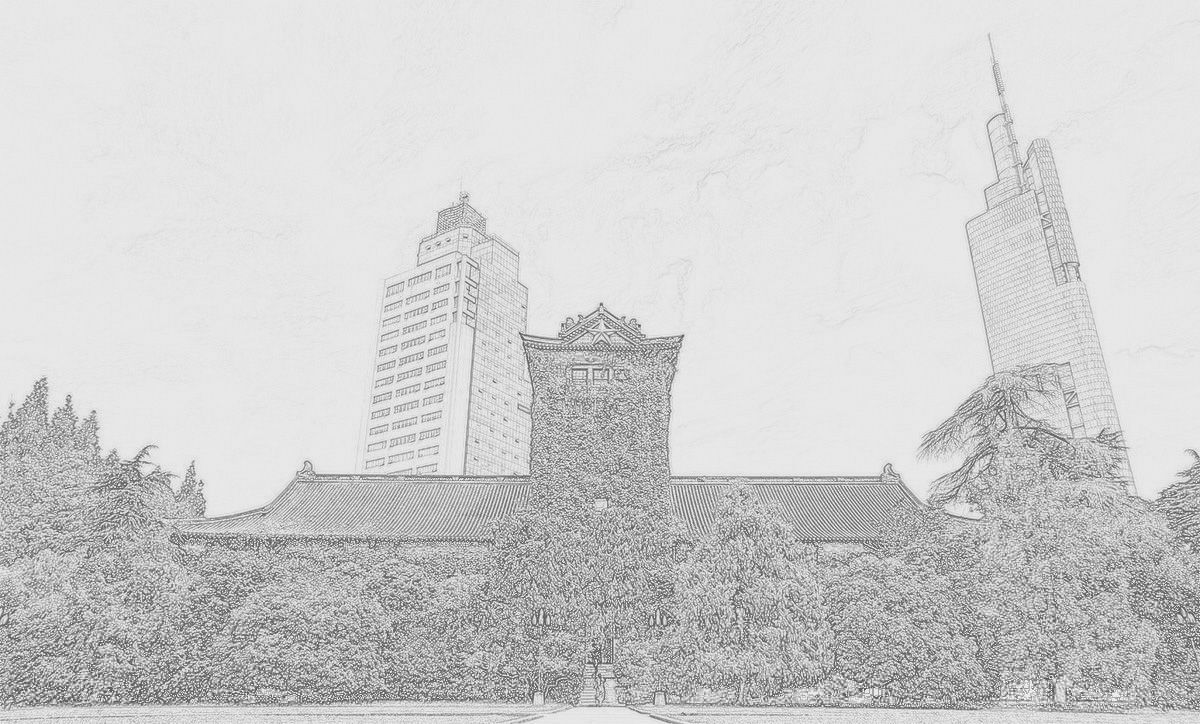
\includegraphics[width=\paperwidth,height=\paperheight]{pic/北大楼.jpg}};
    \end{tikzpicture}
    }

%   普通页背景图
\setbeamertemplate{background canvas}
    {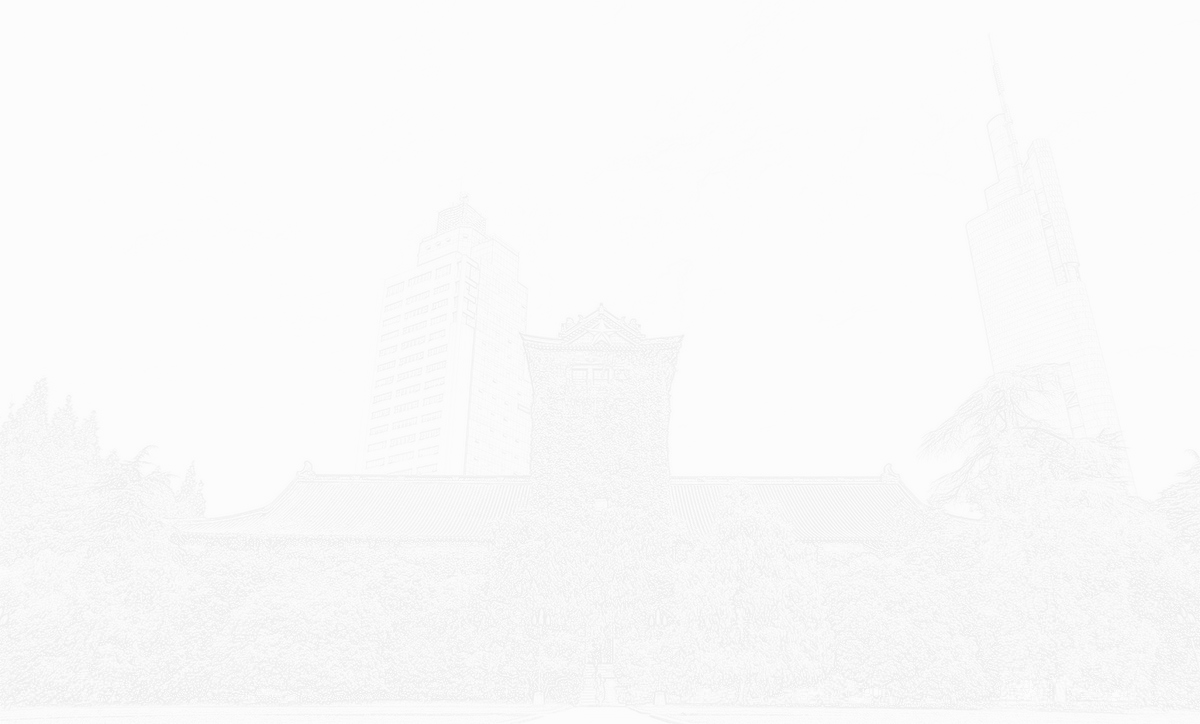
\includegraphics[width=\paperwidth, height=\paperheight]{pic/北大楼10.png}}

%   导航栏
\setbeamertemplate{navigation symbols}{}

%   页标题栏
\setbeamerfont{frametitle}{family=\songti, series=\bfseries, size=\normalsize}
\setbeamercolor{frametitle}{fg=NJU_purple, bg=}
\setbeamertemplate{frametitle}{%
    \leavevmode %   离开垂直模式
    \hbox{%
    \begin{beamercolorbox}[wd=\paperwidth, ht=2.5ex, dp=1ex, left]
        {frametitle}\usebeamerfont{frametitle}
        \hspace*{2pt}\insertframetitle\hspace*{2pt}
    \end{beamercolorbox}%
    }\vskip0pt  %   重返垂直模式
}

%   页眉栏
\setbeamerfont{headline}{family=\songti, series=\bfseries}
\setbeamercolor{section in head/foot}{fg=NJU_purple, bg=black!10}
\setbeamertemplate{headline}{%
    \begin{beamercolorbox}[wd=\paperwidth, ht=6ex, dp=1ex, left] 
        {section in head/foot}\usebeamerfont{headline}
        \vskip2pt\insertnavigation{\paperwidth}\vskip2pt
    \end{beamercolorbox}%\
}

%   页脚栏
\setbeamerfont{shortinstitute in head/foot}{family=\songti}
\setbeamerfont{subtitle in head/foot}{family=\songti}
\setbeamerfont{shortauthor in head/foot}{family=\songti}
\setbeamercolor{shortinstitute in head/foot}{fg=white, bg=NJU_purple}
\setbeamercolor{subtitle in head/foot}{fg=NJU_purple, bg=black!10}
\setbeamercolor{shortauthor in head/foot}{fg=white, bg=NJU_purple}
\setbeamertemplate{footline}{%
    \leavevmode %   离开垂直模式
    \hbox{%
    \begin{beamercolorbox}[wd=.3\paperwidth, ht=3ex, dp=1ex, left] 
        {shortinstitute in head/foot}\usebeamerfont{shortinstitute in head/foot}
        \hspace*{1em}\textbf{\insertshortinstitute}\hspace*{1em}
    \end{beamercolorbox}%
    \begin{beamercolorbox}[wd=.4\paperwidth, ht=3ex, dp=1ex, center]
        {subtitle in head/foot}\usebeamerfont{subtitle in head/foot}
        \hspace*{1em}\textbf{\insertsubtitle}\hspace*{1em}
    \end{beamercolorbox}%
    \begin{beamercolorbox}[wd=.3\paperwidth, ht=3ex, dp=1ex, right]
        {shortauthor in head/foot}\usebeamerfont{shortauthor in head/foot}
        \hspace*{1em}\textbf{\insertshortauthor}\hspace*{1em}
    \end{beamercolorbox}% 
    }\vskip0pt   %   重返垂直模式
}

%   列表
% \setbeamertemplate{itemize items}[circle]
% \setbeamertemplate{enumerate items}[default]
\usepackage{enumitem}
\setlist[itemize]{leftmargin=2em, rightmargin=0em, labelsep=3ex, listparindent=\parindent, itemindent=0em}
\setlist[itemize, 1]{label=\color{NJU_purple}\normalsize$\bullet$}
\setlist[itemize, 2]{label=\color{NJU_purple}\small$\bullet$}
\setlist[itemize, 3]{label=\color{NJU_purple}\footnotesize$\bullet$}
\setlist[enumerate]{leftmargin=2em, rightmargin=0em, labelsep=3ex, listparindent=\parindent, itemindent=0em}
\setlist[enumerate, 1]{label=\color{NJU_purple}\arabic*, font=\normalsize}
\setlist[enumerate, 2]{label=\color{NJU_purple}\arabic*., font=\small}
\setlist[enumerate, 3]{label=\color{NJU_purple}(\arabic*), font=\footnotesize}

%   题注:表头图尾
\usepackage{graphicx}
\usepackage{caption}
\captionsetup[table]{position=top, skip={3pt}}
\captionsetup[figure]{position=bottom, skip={6pt}}
\setbeamertemplate{caption}[numbered]
\numberwithin{figure}{section}
\numberwithin{table}{section}
\numberwithin{equation}{section}
\usepackage{subcaption}
%   块
\setbeamertemplate{blocks}[rounded][shadow=true]
\def\qedsymbol{}                        %   取消证明模块“证毕”(QED)结尾
\usepackage{bm}


%%%%%%%%%%%%%%%%%%%%%%%%%%%%%%%%%%%%%%%%%%%%%%%%%%%%%%%%%%%%%%%%%%%%%%%%%%%%%%%%%%%%%%%%%%%%%%%%%%%%

% overleaf 支持的中文字体
% https://cn.overleaf.com/learn/latex/Questions/Which_OTF_or_TTF_fonts_are_supported_via_fontspec%3F#Chinese

% 使用 XeLaTeX 编译
\usepackage{xeCJK}
\usepackage{fontspec}

% 设置英文字体(macOS 自带字体)
\setmainfont{Times New Roman}          % 正文西文
\setsansfont{Helvetica Neue}           % 无衬线西文
\setmonofont{Menlo}                    % 等宽字体

% 设置中文字体(macOS 自带中文字体)
\setCJKmainfont[
  BoldFont = {Heiti SC},
  ItalicFont = {Songti SC}
]{Songti SC}

% 定义中文字体宏(用于 beamer 设置中)
\newcommand{\songti}{\CJKfamily{song}}  % 会默认使用 PingFang,但你也可以替换
\newcommand{\kaishu}{\CJKfamily{kai}}  % 楷体(如果用不到可省略)

% 设置 beamer 字体
\setbeamerfont{title}{family=\kaishu, series=\bfseries, size=\large}
\setbeamerfont{subtitle}{family=\songti, series=\bfseries, size={\fontsize{24}{28}\selectfont}}
\setbeamerfont{author}{family=\songti, series=\bfseries, size=\large}
\setbeamerfont{institute}{family=\songti, series=\bfseries, size=\normalsize}
\setbeamerfont{date}{family=\songti, series=\bfseries, size=\normalsize}
\setbeamerfont{frametitle}{family=\songti, series=\bfseries, size={\fontsize{14}{16}\selectfont}}

%%%%%%%%%%%%%%%%%%%%%%%%%%%%%%%%%%%%%%%%%%%%%%%%%%%%%%%%%%%%%%%%%%%%%%%%%%%%%%%%%%%%%%%%%%%%%%%%%%%%

\usepackage{color,xcolor}

\setbeamercolor{itemize item}{fg=NJU_purple!80, bg=white}
\setbeamercolor{itemize subitem}{fg=NJU_purple!80, bg=white}
\setbeamercolor{itemize subsubitem}{fg=NJU_purple!80, bg=white}

\setbeamercolor{enumerate item}{fg=NJU_purple!80}
\setbeamercolor{enumerate subitem}{fg=NJU_purple!80}
\setbeamercolor{enumerate subsubitem}{fg=NJU_purple!80}

\setbeamercolor{title}{fg=white, bg=NJU_purple}
\setbeamercolor{subtitle}{fg=white, bg=NJU_purple}
\setbeamercolor{author}{fg=NJU_golden}
\setbeamercolor{institute}{fg=NJU_golden}
\setbeamercolor{date}{fg=NJU_golden}

\xdefinecolor{NJU_purple}{rgb}{0.412,0.027,0.353}   %   南大紫
\xdefinecolor{NJU_golden}{rgb}{0.722,0.561,0.298}   %   南大金  #D7B758
\xdefinecolor{NJU_yellow}{cmyk}{0.00, 0.30, 1.00, 0.00}
\xdefinecolor{NJU_pink}{cmyk}{0.05, 1.00, 0.55, 0.00}
\xdefinecolor{NJU_blue}{cmyk}{0.80, 0.50, 0.00, 0.00}

\usepackage[T1]{fontenc}



